\documentclass{beamer}
\usetheme{metropolis}
\usepackage{subcaption}

% Configuration des couleurs modernes
\definecolor{myblue}{RGB}{173, 216, 230} % Bleu pastel
\definecolor{mymagenta}{RGB}{238, 130, 238} % Magenta doux
\definecolor{mywhite}{RGB}{255, 255, 255} % Blanc pur
\definecolor{mygray}{RGB}{245, 245, 245} % Gris clair
\definecolor{darkblue}{RGB}{25, 25, 112} % Bleu foncé
\definecolor{darkviolet}{RGB}{148, 0, 211} % Violet foncé
\definecolor{goldenrod}{RGB}{218, 165, 32} % Or doux

% Arrière-plan sobre et clair
\usepackage{tikz}

\addtobeamertemplate{background canvas}{}{
    \begin{tikzpicture}[remember picture, overlay]
        \fill[mywhite] (current page.south west) rectangle (current page.north east);
        \begin{scope}[blend mode=overlay]
            \shade[inner color=myblue!60, outer color=mywhite] (current page.south west) rectangle (current page.north east);
            \shade[inner color=mymagenta!60, outer color=mywhite] (current page.north east) rectangle (current page.south west);
        \end{scope}
    \end{tikzpicture}
}

% Personnalisation des couleurs dans metropolis
\setbeamercolor{normal text}{fg=black}
\setbeamercolor{frametitle}{bg=mywhite, fg=black}
\setbeamercolor{title separator}{fg=mymagenta}
\setbeamercolor{progress bar}{fg=myblue, bg=mymagenta}
\setbeamercolor{block title}{bg=myblue, fg=black}
\setbeamercolor{block body}{bg=mywhite, fg=black}
\setbeamercolor{alerted text}{fg=darkviolet!70}

% Personnalisation des typos
\setbeamerfont{frametitle}{size=\Large,series=\bfseries}
\setbeamerfont{title}{size=\Huge,series=\bfseries}

% Apparence des transitions entre les frames
\metroset{progressbar=frametitle,numbering=fraction}

% Commande pour ajuster le séparateur du titre
\metroset{titleformat frame=smallcaps}

% Début du document
\begin{document}

\title{Diffusion Model}
\subtitle{Computer Vision - Project}
\author{Clément, Grégoire, Nathan}
\date{\today}

\maketitle
\begin{frame}{What is Diffusion ?}
    \begin{minipage}[c]{0.5\textwidth}
        \centering
        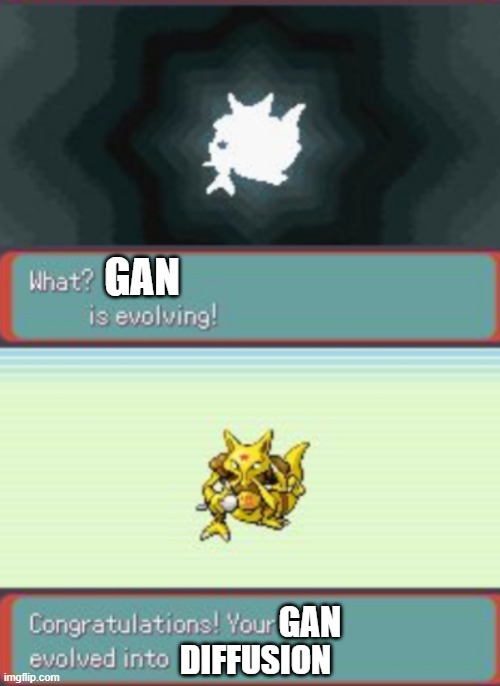
\includegraphics[width=\textwidth]{imgs/evolution_meme.jpg}
    \end{minipage}%
    \hfill
    \begin{minipage}[c]{0.35\textwidth}
        \alert{Diffusion} is the \alert{state-of-the-art} generative process to generate images for creating \alert{new images near the original one}.  
        It also allows to \alert{generate images from text}.
    \end{minipage}
\end{frame}

\section{First generation: Denoising Diffusion Probabilistic Models}



\begin{frame}{General Idea}
    \only<1>{
    \begin{figure}
        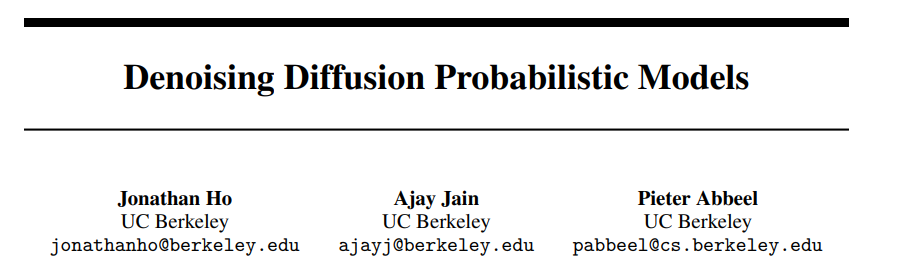
\includegraphics[width=0.8\textwidth]{imgs/ddpm_paper.png}
    \end{figure}
    }
    \only<2>{Consider the set of \alert{hand-written digits $D$}. Can you give a probability distribution $q$ such that \alert{$x \sim q(x)$ ?}
    \begin{figure}
        \centering
            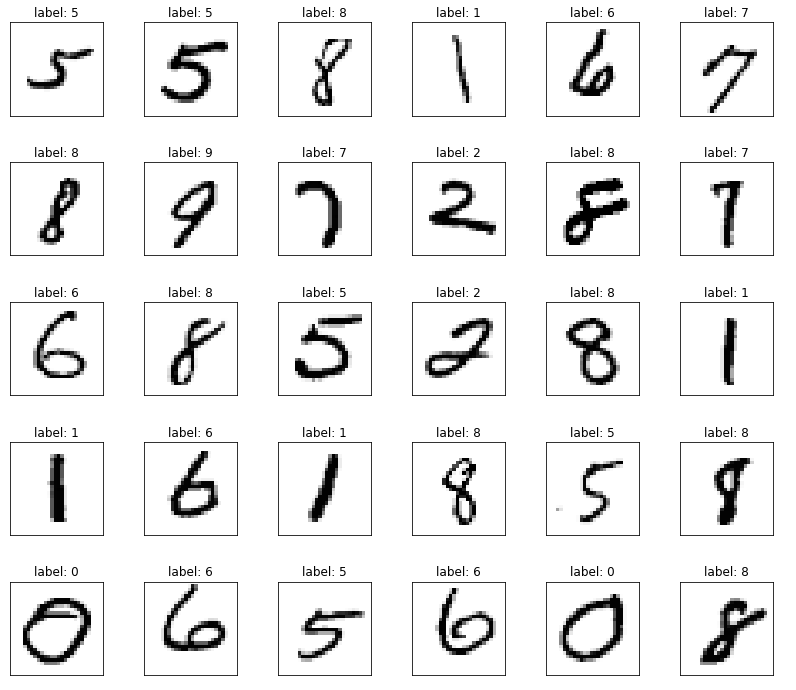
\includegraphics[width=0.5\textwidth]{imgs/mnist_sample_digits.png}
            \caption{Source: ludwig.ai}
        \end{figure}
    }
    \only<3->{
        Consider the set of \alert{hand-written digits $D$}. It is hard to find $q$ such that \alert{$x \sim q(x)$}, we need a \alert{clever way to sample hand-written digits}. Consider the following process:
        \begin{figure}
            \centering
            \begin{minipage}{0.2\textwidth}
                \centering
                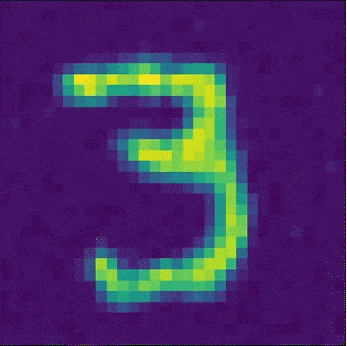
\includegraphics[width=\textwidth]{imgs/frame1.png}
            \end{minipage}%
            \only<4->{
                \begin{minipage}{0.2\textwidth}
                    \centering
                    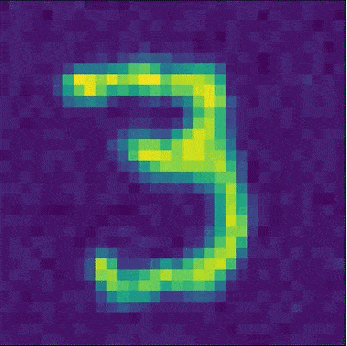
\includegraphics[width=\textwidth]{imgs/frame2.png}
                \end{minipage}
                \only<5->{
                    \begin{minipage}{0.2\textwidth}
                        \centering
                        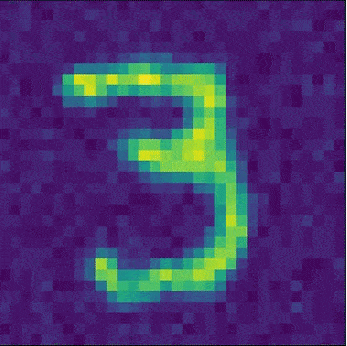
\includegraphics[width=\textwidth]{imgs/frame3.png}
                    \end{minipage}
                    \only<6->{
                    \begin{minipage}{0.2\textwidth}
                        \centering
                        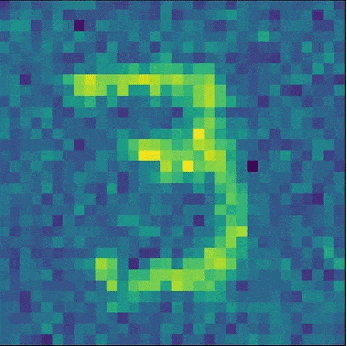
\includegraphics[width=\textwidth]{imgs/frame52.png}
                    \end{minipage}
                    \only<7->{
                    \begin{minipage}{0.2\textwidth}
                        \centering
                        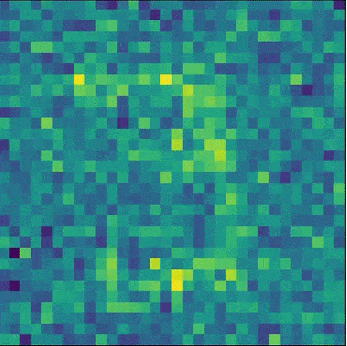
\includegraphics[width=\textwidth]{imgs/framelot.png}
                    \end{minipage}
                    \only<8->{
                    \begin{minipage}{0.2\textwidth}
                        \centering
                        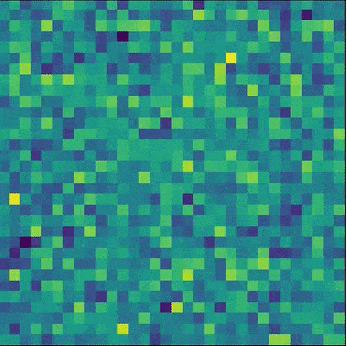
\includegraphics[width=\textwidth]{imgs/framerandom.png}
                    \end{minipage}
                }
                }
                }
                }
                
            }
        \end{figure}
        \only<9->{
            Formally: $q(x_{t+1} \mid x_t) := \mathcal{N}(x_{t+1}; \sqrt{1 - \beta_t} x_t, \beta_t I)$ for some schedule $(\beta_t)_t$. Can we \alert{learn to reverse this process} ?
        }
    }
\end{frame}



\begin{frame}{What we want to learn}
    Given a noisy image $x_t$, we \alert{train a model to predict $x_{t-1}$}.
    \begin{figure}
        \centering
        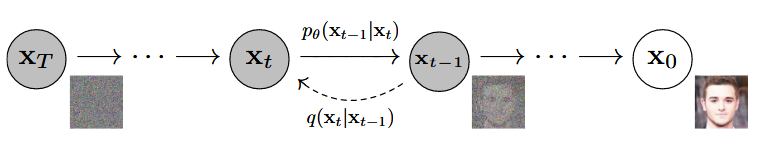
\includegraphics[width= \textwidth]{imgs/ho_diffusion_process.png}
    \end{figure}

    \only<2->{
    \begin{itemize}
        \only<2->{\item{Given a \alert{noisy image $x_t$} and $t$, we sample according to $p_\theta (x_{t-1} \mid x_t) := \mathcal{N}(x_{t-1} ; \mu_\theta(x_t,t), \Sigma_\theta (x_t,t))$}.}
    \end{itemize}
    }
\end{frame}

\begin{frame}{Decreasing training data generation cost}
    Given a data image \(x_0\), computing \(x_t\) takes \alert{\(t\) samplings on \(q\)}. But a \alert{simple trick} allows us to do it in only one step.

    \only<1>{ 
    Remember that \(q(x_{t+1} \mid x_t) := \mathcal{N}(x_{t+1}; \sqrt{1 - \beta_t} x_t, \beta_t I)\). Let \(\alert{\alpha_t} = 1 - \beta_t\) and \(\alert{\bar{\alpha_t}} = \prod_{i=1}^t \alpha_i\).
    \begin{align*}
    x_t &= \sqrt{\alpha_t} x_{t-1} + \sqrt{1 - \alpha_t} \epsilon_{t-1} \\
    &= \sqrt{\alpha_t} \sqrt{\alpha_{t-1}} x_{t-2} + \sqrt{\alpha_t} \sqrt{1 - \alpha_{t-1}} \epsilon_{t-1} + \sqrt{1 - \alpha_t} \epsilon_{t-1} \\
    &= \sqrt{\alpha_t \alpha_{t-1}} x_{t-2} + \sqrt{\alpha_t (1 - \alpha_{t-1}) + (1 - \alpha_t)} \bar{\epsilon_t} \\ 
    &= \sqrt{\alpha_t \alpha_{t-1}} x_{t-2} + \sqrt{1 - \alpha_t \alpha_{t-1}} \bar{\epsilon_t}
    \end{align*}
    Let \(G_1 \sim \mathcal{N}(0,\sigma_1^2 I)\), \(G_2 \sim \mathcal{N}(0,\sigma_2^2 I)\), the sum of them gives \(g_2 \sim \mathcal{N}(0,(\sigma_1^2 + \sigma_2^2) I)\).
    }
    \only<2>{
    We have \alert{\(x_t = \sqrt{\bar{\alpha_t}} x_0 + \sqrt{1 - \bar{\alpha_t}} \epsilon\)}.
    }
\end{frame}


\begin{frame}{Training}
\only<1>{
For now, our model is learning $\mu$ and $\Sigma$, i.e. we sample according to 
\begin{align*}
p_\theta (x_{t-1} \mid x_t) := \mathcal{N}(x_{t-1} ; \mu_\theta(x_t,t), \Sigma_\theta (x_t,t))
\end{align*}
They fixed \alert{fixing $\Sigma_\theta$} to a constant to simplify computations. So,}
\begin{align*}
    p_\theta (x_{t-1} \mid x_t) := \mathcal{N}(x_{t-1} ; \mu_\theta(x_t,t), \sigma_t I)
\end{align*}
    \only<2->{Using negative log likelihood, approximations and computations, we want to minimize:
    \begin{align*}
    E_q \left[\frac{1}{2 \sigma_t^2} \|\tilde{\mu}_t(x_t,x_0) - \mu_\theta(x_t,t)\|^2\right]
    \end{align*} where $\tilde{\mu}$ is the optimal mean \alert{that depends on $x_0$ \only<3>{which we don't know}}.
    }\only<3>{We can also have $\epsilon$ using \begin{align*}
    E_q \left[ \frac{\beta_t^2}{2 \sigma_t^2 \alpha_t (1 - \bar{\alpha_t})} \|\epsilon - \epsilon_\theta (\sqrt{\bar{\alpha_t}} x_0 + \sqrt{1 - \bar{\alpha_t}} \epsilon, t)\|\right]
    \end{align*}}
    
\end{frame}


\begin{frame}{Our results - Gaussian}
    We have started with \alert{Gaussian generation}\only<1>{:
    \begin{figure}
        \centering
        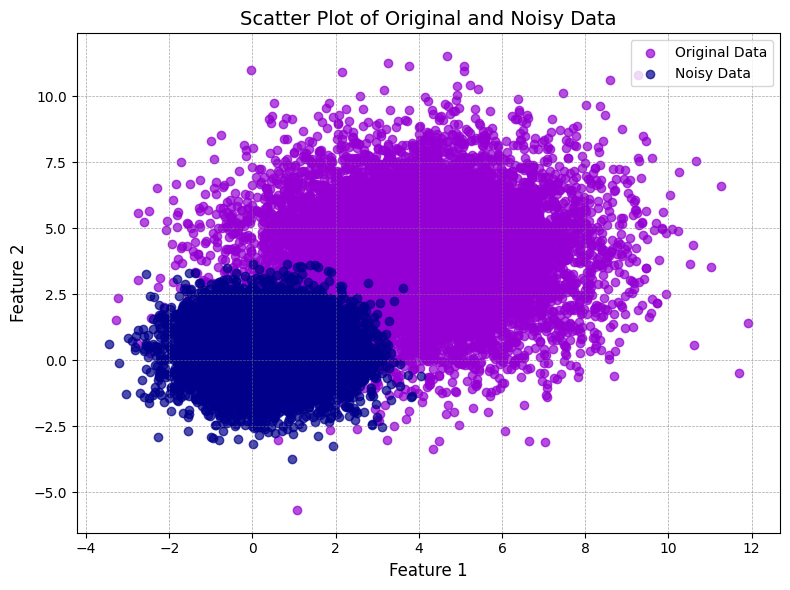
\includegraphics[width= 0.8\textwidth]{imgs/ho_implementation_init.png}
    \end{figure}
    }\only<2>{ and got satisfying results:
    \begin{figure}
        \centering
        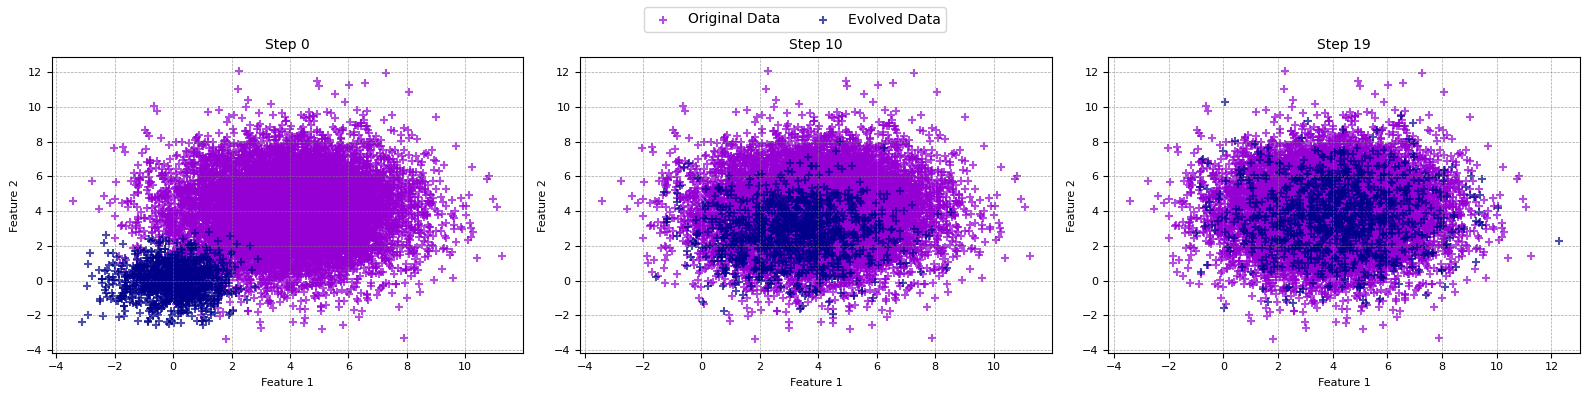
\includegraphics[width= \textwidth]{imgs/ho_gaussian_res.png}
    \end{figure}
    }
\end{frame}

\begin{frame}{Our results - Spirale}
    Then we moved to a more complicated dataset, \alert{Spirale generation}\only<1>{:
    \begin{figure}
        \centering
        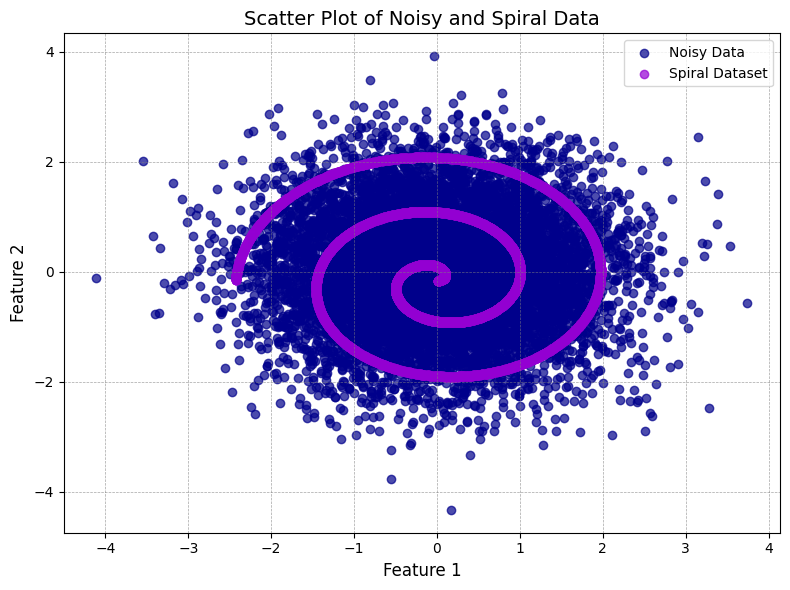
\includegraphics[width= 0.8\textwidth]{imgs/spirale_dataset.png}
    \end{figure}}\only<2>{ and also got satisfying results:
    \begin{figure}
        \centering
        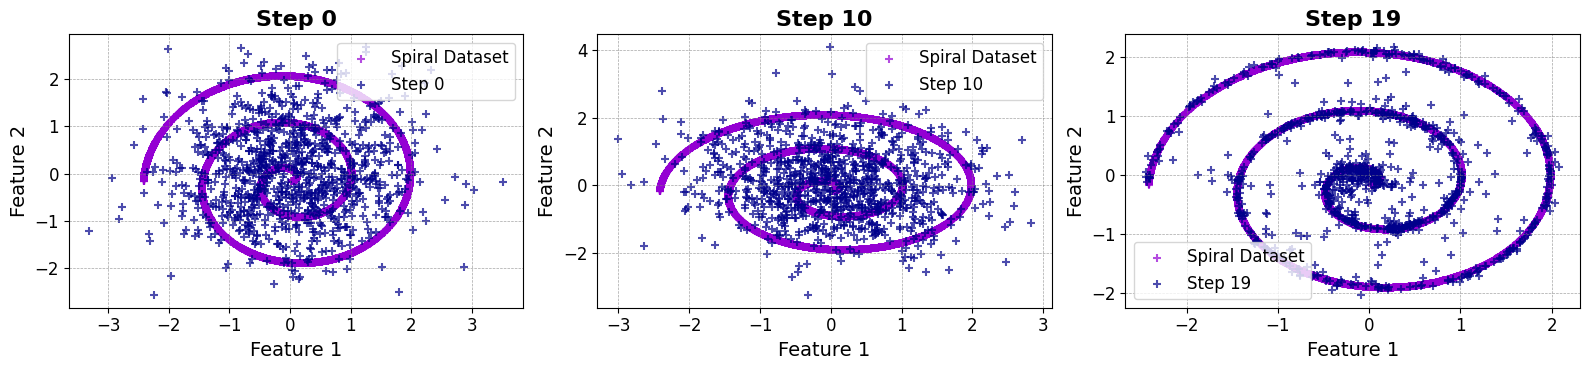
\includegraphics[width= \textwidth]{imgs/res_spirale.png}
    \end{figure}
    }
    
\end{frame}


\begin{frame}{Generating Images}
    We need a \alert{model powerful enough to predict $\epsilon$} (or $\mu$) for \alert{2D images} (the size of $\epsilon$), for this we use \alert{UNet}.

    \begin{figure}
        \centering
        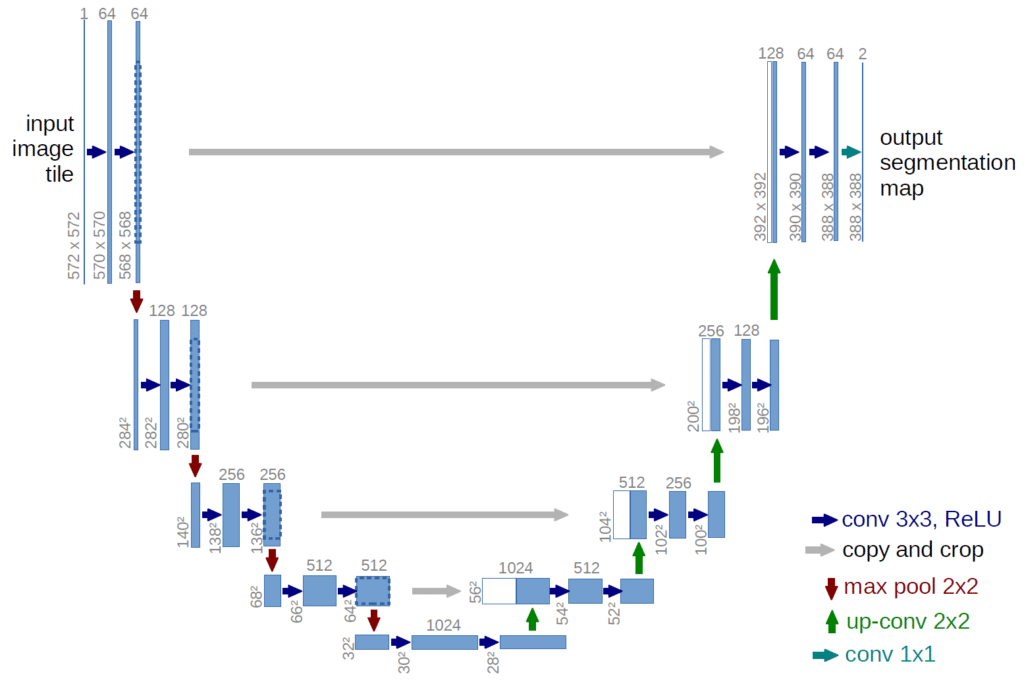
\includegraphics[width = 0.8\textwidth]{imgs/unet-architecture.png}
    \end{figure}
\end{frame}
\begin{frame}{Our results - MNIST Generation}
    \begin{figure}
        \centering
        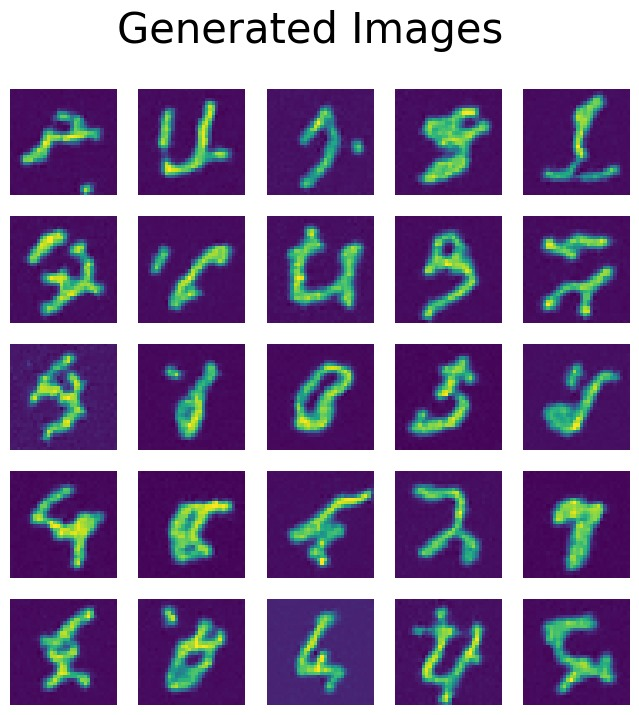
\includegraphics[width = 0.65\textwidth]{imgs/mnist_res.jpg}
    \end{figure}
\end{frame}
\section{Amelioration}

\begin{frame}{Accelerating generation}
    \begin{figure}
        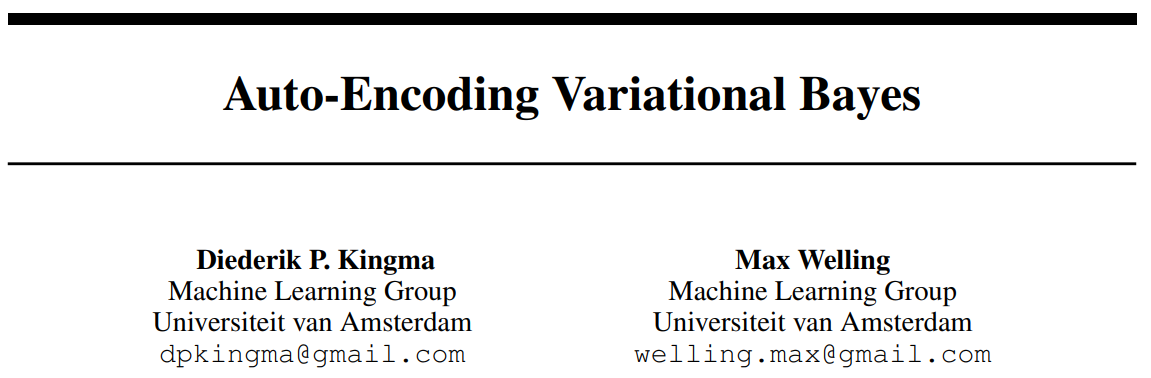
\includegraphics[width=\textwidth]{imgs/papier_accelerer.png}
    \end{figure}
    Imagine that you have $T = 10,000$. You \alert{can not do 10,000 steps to generate one image}. But, using the \alert{reparametrization trick}:

    \begin{align*}
        x_{T} &= x_0 + \sigma_{T,0} \epsilon_{T} \Rightarrow \alert{\tilde{x_0}}\\
        x_{T-k} &= \tilde{x_0} + \sigma_{T-k,0} \epsilon_{T-k}
    \end{align*}

    So we can \alert{generate with $T/k$ steps}.
    
\end{frame}

\begin{frame}{OpenAI's incrementation}
    \begin{figure}
        \centering
        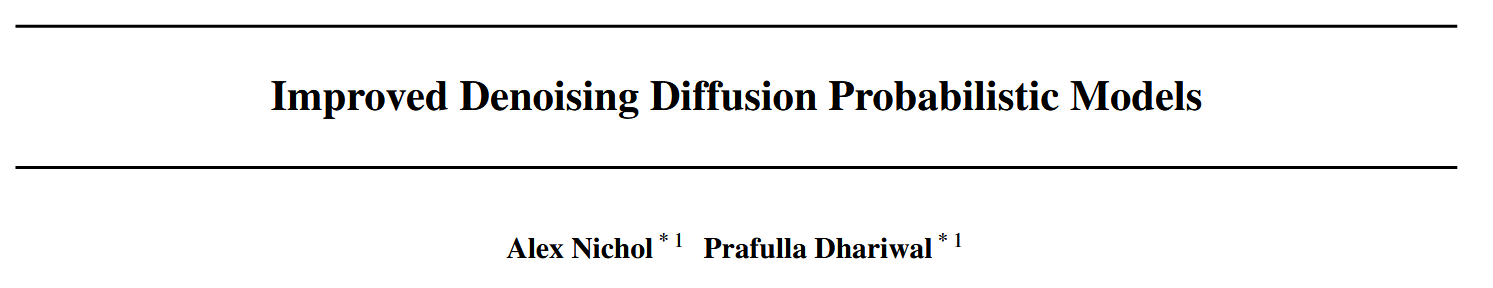
\includegraphics[width= \textwidth]{imgs/paper_gen2.png}
    \end{figure}

\uncover<2->{Recall that:
\begin{itemize}
    \item \uncover<2->{$\Sigma_\theta$ was \alert{set to a constant},}
    \item \uncover<3->{The training loss was a \alert{simplified} version of reality.}
\end{itemize}

\uncover<4>{This paper \alert{tackle these problems}.}
}
\end{frame}

\begin{frame}{How to modelize $\Sigma_\theta$}
    \only<1-4>{
Ho et al. fixed $\Sigma_\theta(x_t,t) = \sigma_t^2 I$ with: 
\begin{itemize}
    \item $\sigma_t^2 = \beta_t $ optimal if $x_0 \sim \mathcal{N}(0,I)$,
    \uncover<2->{
        \item $\sigma_t^2 = \bar{\beta_t} $ optimal if $x_0$ is a point.
    }
\end{itemize}
    }
\uncover<3->{
    
Hence for each $t$, we know that \alert{$\Sigma^* (x_,t)$ is between $\beta_t$ and $\bar{\beta_t}$}.}
\uncover<4->{
    
Ho et al. have found that the impact is negligeable\only<4-5>{...}\only<6->{. But it depends of \alert{other hyperparameters}.}
\only<5>{
    \begin{figure}
        \centering
        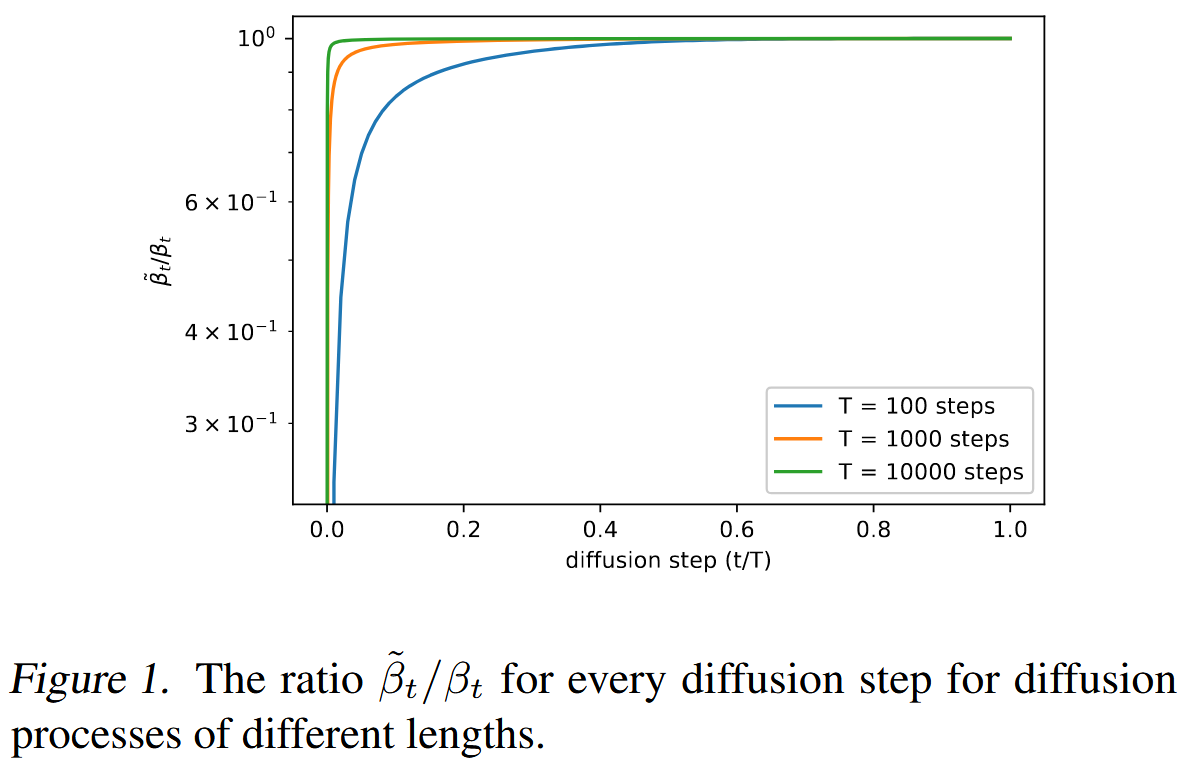
\includegraphics[width= 0.8\textwidth]{imgs/ratio_tilde_et_normal.png}
    \end{figure}
}
\only<6>{
    
Hence, they \alert{interpolate between the two extreme values}, and let the \alert{model learn $v(t)$}:
\begin{align*}
    \Sigma_\theta(x_t,t) := \exp(v_\theta (t) \log(\beta_t) + (1 - v_\theta (t)) \log(\bar{\beta}_t))
\end{align*}
}
}

\end{frame}

\begin{frame}{Changing the Loss}
    In the paper of Ho, they use the loss $L_{simple}$, a simplified version of $L_{LVB}$, that only affects $\mu_\theta$.
    
    \uncover<2->{Optimizing $L_{simple}$ \alert{performs well for FID}, but \alert{poorly} for log-likelihood metric.}
    \uncover<3->{
        
    $L_{LVB}$ affects $\Sigma_\theta$ but \alert{increasing log-likelihood score can increase FID}, hence we \alert{need a trade-of}.}

    \uncover<4->{
        They train on 
        \begin{align*}
            L = L_{simple} + \lambda L_{LVB}
        \end{align*}
    }

    \uncover<5>{This loss is prone to \alert{gradient exploding} and we need \alert{importance sampling} to implement it.}
\end{frame}


\section{Classifier Guidance}

\begin{frame}{Importance of labels}
    Let's get back to hand-written digits generation:
    \only<-2>{
    \begin{figure}
        \centering
            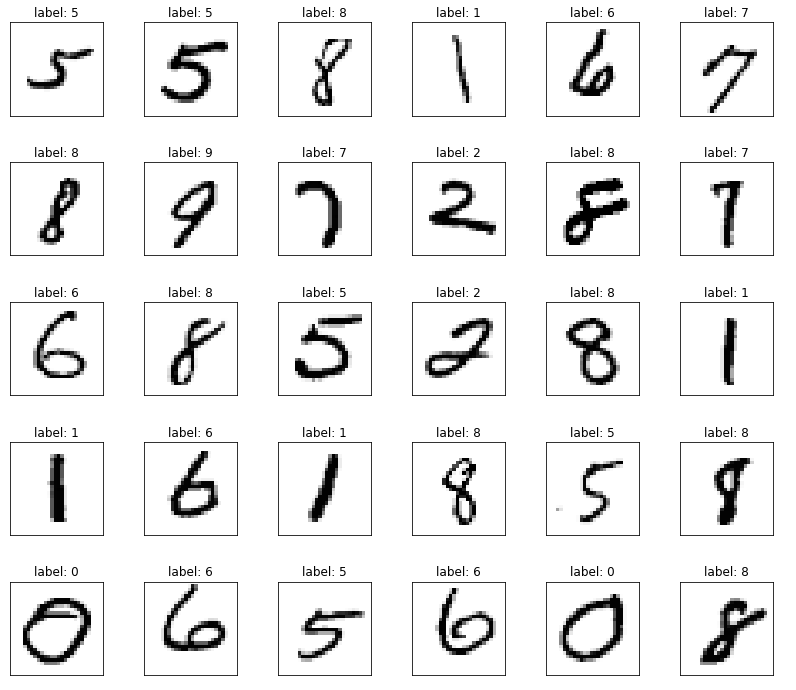
\includegraphics[width=0.4\textwidth]{imgs/mnist_sample_digits.png}
            \caption{Source: ludwig.ai}
    \end{figure}
    }
    \only<2>{A DDPM can \alert{generate new images that look like digits}, but the \alert{model can't distinguish a mix of two digits and a real digit}.}
    \only<3->{

        If we have a \alert{classifer} that gives $p_\phi (y \mid x_t)$, we can \alert{sample using} \begin{align*}
            p_{\theta,\phi}(x_t \mid x_{t+1},y) = Z p_\theta(x_t \mid x_{t+1}) p_\phi(y \mid x_t)
        \end{align*} This way if we set $y=3$, we can \alert{trick our model to generate somthing that looks like a 3}.
    }

\end{frame}

\begin{frame}{Langevin Dynamics}
    Given $x_0 \sim \pi(x)$ an unknown distribution, if we iterate through $x_{i+1} \leftarrow x_i + \epsilon \nabla_x \log p(x) + \sqrt{2 \epsilon} z_i$ with $\epsilon \rightarrow 0$ and $z_i \sim \mathcal{N}(0,I)$, we can sample from $p(x)$.

    \only<2-5>{
    \begin{figure}[ht]
        \centering
        \only<2>{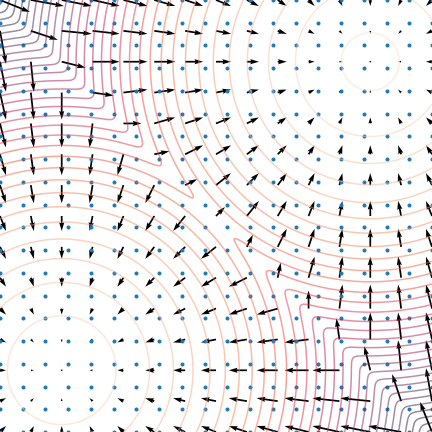
\includegraphics[width=0.5\textwidth]{imgs/langevin0.png}}
        \only<3>{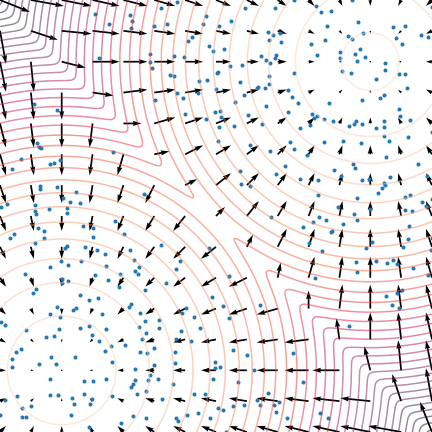
\includegraphics[width=0.5\textwidth]{imgs/langevin1.png}}
        \only<4>{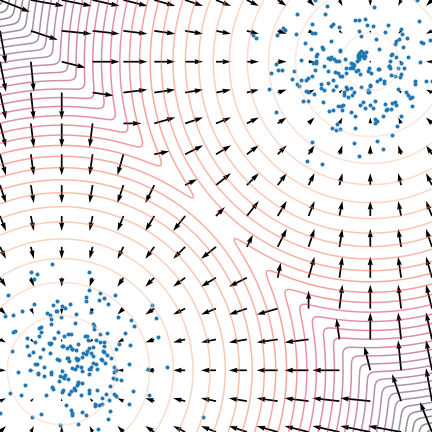
\includegraphics[width=0.5\textwidth]{imgs/langevin3.png}}
        \only<5>{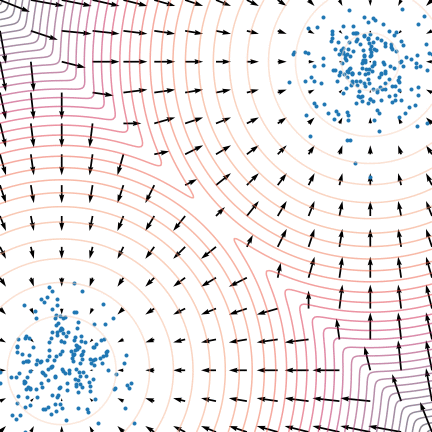
\includegraphics[width=0.5\textwidth]{imgs/langevin4.png}}
        \caption{Visualizations from Yang Song's work.}
        \label{fig:yang_song}
    \end{figure}  
    }  

    \only<6->{So we \alert{need to know $\nabla_x \log p(x)$}, but don't need to know $p(x)$.}

    \only<7->{From the classifier $p_\phi$, one \alert{can get an approximation of $\nabla_x \log p(x)$}.}
    
\end{frame}

\begin{frame}{Low vs High temperature}
    \begin{figure}
        \centering
            
\includegraphics[width=\textwidth]{imgs/guided_effect.png}
            \caption{Classifier-free Diffusion Guidance}
    \end{figure}

\only<2->{
\begin{itemize}
    \item{Low-temperature optimizes \alert{FID score}}
    \only<3->{\item{High-temperature optimizes \alert{Inception score}}}
    \end{itemize}
}

\only<4>{
    We can do a \alert{trade-of} by following more $p_\phi$ or $p_\theta$ between \alert{exploration and distance to the original distribution}.
}

\end{frame}

\section{GLIDE: draw what you prompt}

\begin{frame}{Classifier-Free Guidance}
Previous guidance \alert{need a trained classifier}. They define:
\begin{itemize}
    \item{An \alert{unconditional} DDPM, that predicts $p_\theta (z)$.}
    \item{A \alert{conditional} DPPM, that predicts $p_\theta(z \mid c)$.}
\end{itemize}
\only<2>{
    Rather than using $p_\phi$, they train both models simultanously and \alert{use the gradient of $p_\theta (z \mid c)$ to estimate $\nabla \log p(z \mid c)$}.
}
\end{frame}

\begin{frame}{CLIP}
    \only<-2>{To force a \alert{label $c$}, we train a model that estimates the probability for \alert{$x$ to be of class $c$, and uses its gradient}.}

    \only<2->{To force a \alert{sentence $c$}, we train a model that estimates the distance between \alert{$x$ and the sentence $c$, and uses its gradient}.}

    \only<3->{
        \begin{figure}
            \centering
                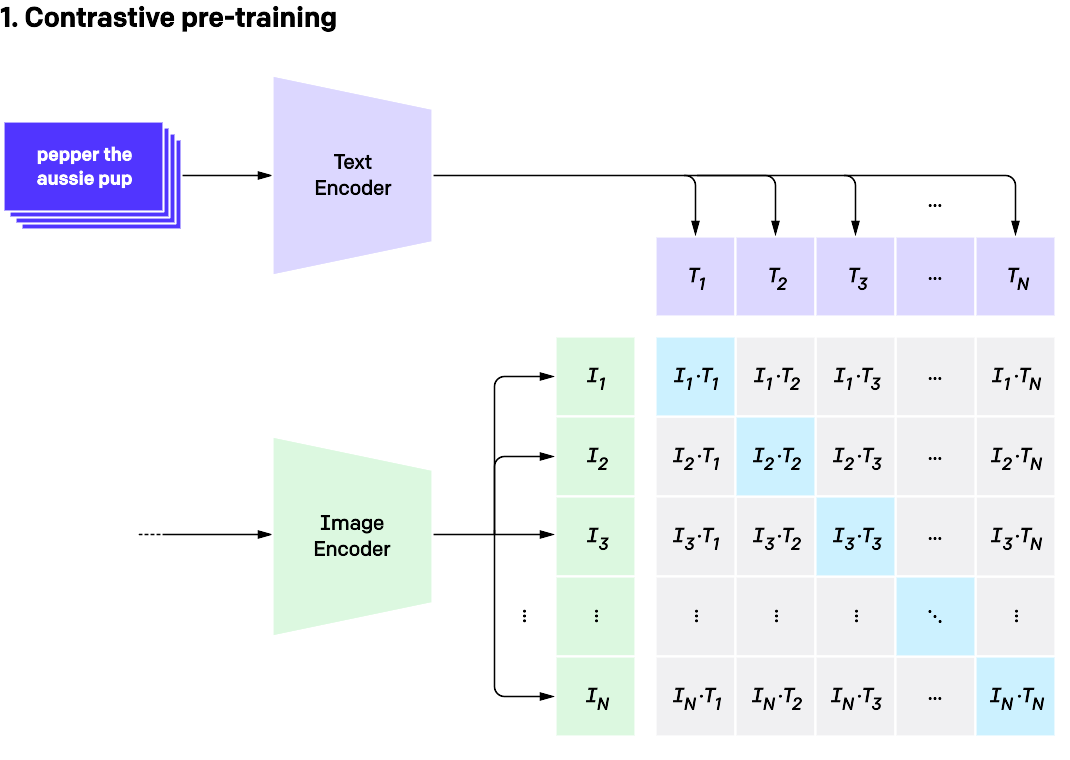
\includegraphics[width=0.8\textwidth]{imgs/clip.png}
                \caption{How to compare an image and a text}
        \end{figure}
    }
\end{frame}

\begin{frame}{Results (OpenAI GLIDE)}
    \begin{figure}
        \centering
            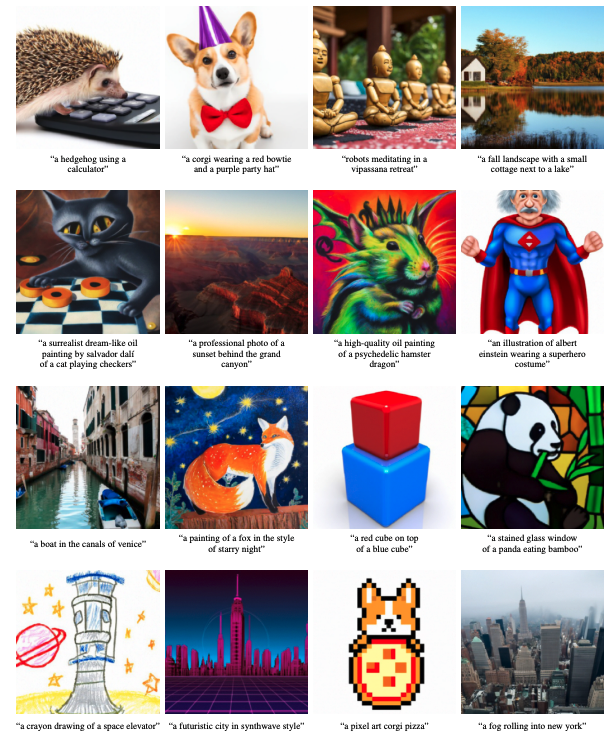
\includegraphics[width=0.8\textwidth]{imgs/glide_result.png}
    \end{figure}
\end{frame}


\section{State-of-the-art brief review}

\begin{frame}{ControlNet}
    \only<1-2>{
GLIDE \alert{accepts} one more input than text: \alert{a mask for inpainting}.

\only<2->{ControlNet generalises it by \alert{adding more optional inputs} (e.g. Cany edges representation / Human Pose / Sketch).}
    }

\only<3>{
    \begin{figure}
        \centering
            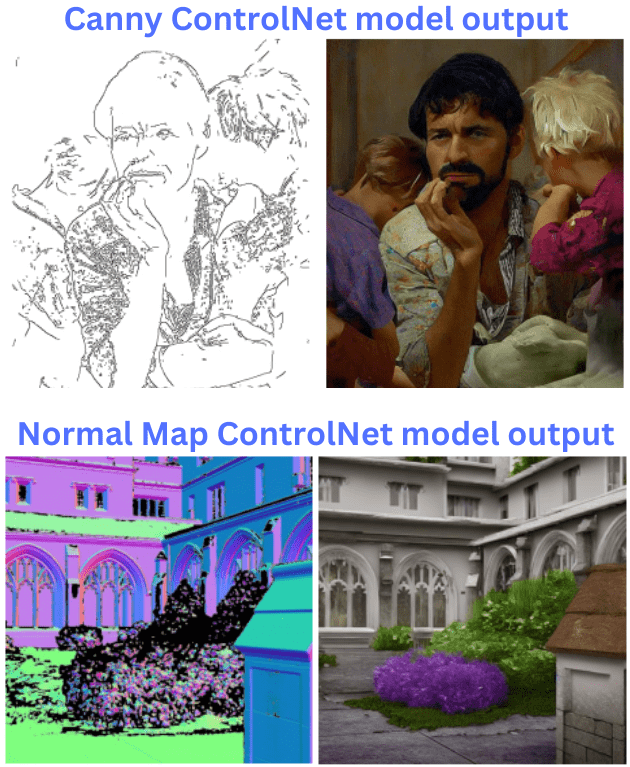
\includegraphics[width=0.6\textwidth]{imgs/controlnet-example.png}
    \end{figure}
}
\end{frame}
\end{document}
